%license:BSD-3-Clause
%copyright-holders:Michele Maione
%============================================================
%
%	Piattaforma di cloud gaming per giochi arcade
%
%============================================================

\chapter{Architettura del sistema}
In questo capitolo verrà fatta\dots

\section{Sistema proposto}
L'esigenza per la quale nasce questo progetto è far conoscere alle nuove generazioni i videogiochi che hanno fatto la storia e dare la possibilità di poter giocare ancora a macchine che ormai hanno cessato di funzionare per motivi di obsolescenza, sfruttando due tecnologie entrate a far parte della quotidianità, lo streaming e il cloud computing. In questo lavoro si propone la creazione di una piattaforma di cloud gaming, che permette lo streaming audio-video direttamente e su richiesta dei videogiochi, da un server remoto, ad un client (computer, console, telefono). Per far ciò verrà ampliato il software MAME (rilasciato sotto licenza GNU-GPL) che è in grado di emulare oltre 7.000 giochi arcade. Le caratteristiche principali del progetto, che sono state vincolanti nella scelta delle tecnologie da utilizzare, sono la portabilità e la possibilità di utilizzare il sistema senza dover installare software aggiuntivi, e per questi vincoli, lato client, la scelta è ricaduta sul browser web. In Fig. \ref{fig:webprotocols} sono schematizzati i protocolli, i servizi e le API relativi alle tecnologie di streaming per i browser web ad oggi disponibili\cite{Audio_and_video_delivery}, che sono:

\begin{itemize}
	\item WebSocket è un protocollo di comunicazione che fornisce un canale full-duplex su una singola connessione TCP, con una latenza inferiore rispetto ad HLS e DASH;
	\item HTTP Live Streaming (HLS) è il protocollo di streaming ad alta latenza più popolare su HTTP per video on demand (video preregistrato) sviluppato da Apple;
	\item Dynamic Adaptive Streaming over HTTP (DASH) è una tecnica di streaming con bit-rate adattivo del Moving Picture Experts Group (MPEG), che consente lo streaming di alta qualità di contenuti multimediali su protocollo HTTP;
	\item Web Real-Time Communication (WebRTC) è un progetto per la comunicazione in tempo reale basato sul protocollo RTP (Real-time Transport Protocol)\cite{High_Performance_Browser_Networking}.
\end{itemize}

\begin{figure}[H]
	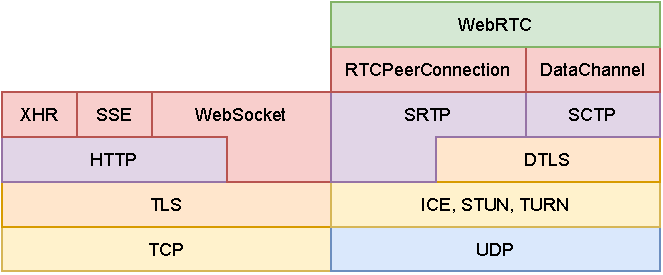
\includegraphics[width=\linewidth]{immagini/webprotocols}
	\caption{API, protocolli e servizi di rete del browser di alto livello}
	\label{fig:webprotocols}
\end{figure}

Il sistema è stato progettato con un'ottica incentrata sull'utilizzo in stand di retro-gaming ad eventi di informatica e videogiochi, da utilizzare quindi sulla rete locale dell'evento con gli utenti connessi tramite WiFi. In questo contesto la differenza di velocità tra TCP e RTP può essere trascurata, e la scelta della tecnologia di streaming da usare è ricaduta su WebSocket perché è un protocollo di comunicazione standardizzato dal 2011, è pienamente supportato da tutti i browser moderni, ha una latenza inferiore rispetto ad HLS e DASH, è semplice da instanziare e non richiede l'utilizzo di protocolli aggiuntivi o configurazioni complesse a differenza di WebRTC.

\begin{figure}[H]
	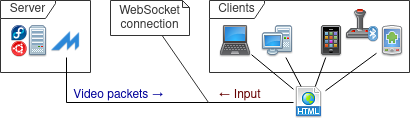
\includegraphics[width=\linewidth]{immagini/proposed_system}
	\caption{Panoramica del sistema}
	\label{fig:proposed_system}
\end{figure}

Come mostrato in Fig. \ref{fig:proposed_system} il sistema è costituito dal server di gioco, che può essere Linux, Windows o macOS, su cui è in esecuzione la versione modificata di MAME ed una pagina HTML5 che funge da front-end. Il programma è in ascolto per connessioni WebSocket con parametri (per es.: il nome del gioco, l'ID del player, l'ID della partita). Una volta stabilita la connessione, il server invia informazioni sulla dimensione e le proporzioni del video e avvia il gioco. Il rendering e il missaggio audio del gioco vengono generati utilizzando la libreria SDL\footnote{SDL: Simple DirectMedia Layer, una libreria multipiattaforma ed open-soure per il multimedia}, codificati e pacchettizzati nel contenitore MPEG-TS\footnote{MPEG-TS: MPEG transport stream, è un contenitore digitale per la trasmissione e l'archiviazione audio-video.} usando la libreria FFmpeg\footnote{FFmpeg è una suite open-source di librerie e programmi per la gestione di video, audio, e altri file multimediali e stream.} e inviati tramite WebSocket al client.

Lato client vari script si occupano di decodificare i dati audio-video ricevuti, catturare e inviare l'input dell'utente, sia dalla tastiera che dal gamepad, al server tramite WebSocket.

\section{MAME}
Lorem ipsum dolor sit amet, consectetur adipiscing elit, sed do eiusmod tempor incididunt ut labore et dolore magna aliqua. Ut enim ad minim veniam, quis nostrud exercitation ullamco laboris nisi ut aliquip ex ea commodo consequat. Duis aute irure dolor in reprehenderit in voluptate velit esse cillum dolore eu fugiat nulla pariatur. Excepteur sint occaecat cupidatat non proident, sunt in culpa qui officia deserunt mollit anim id est laborum.

\subsection{Libs.}
Lorem ipsum dolor sit amet, consectetur adipiscing elit, sed do eiusmod tempor incididunt ut labore et dolore magna aliqua. Ut enim ad minim veniam, quis nostrud exercitation ullamco laboris nisi ut aliquip ex ea commodo consequat. Duis aute irure dolor in reprehenderit in voluptate velit esse cillum dolore eu fugiat nulla pariatur. Excepteur sint occaecat cupidatat non proident, sunt in culpa qui officia deserunt mollit anim id est laborum.

\subsection{Server}
Lorem ipsum dolor sit amet, consectetur adipiscing elit, sed do eiusmod tempor incididunt ut labore et dolore magna aliqua. Ut enim ad minim veniam, quis nostrud exercitation ullamco laboris nisi ut aliquip ex ea commodo consequat. Duis aute irure dolor in reprehenderit in voluptate velit esse cillum dolore eu fugiat nulla pariatur. Excepteur sint occaecat cupidatat non proident, sunt in culpa qui officia deserunt mollit anim id est laborum.

\subsection{SDL renderer} \label{SDL_renderer}
La fase di rendering del MAME inizia creando un contesto di rendering relativo ad una finestra, continua eseguendo la fase di disegno e finisce visualizzado il frame sulla finestra. Le funzioni della libreria SDL utilizzate sono:

\begin{itemize}
	\item CreateRGBSurfaceWithFormat: Crea una superficie RGB specificando il formato pixel da utilizzare;
	\item CreateRenderer: Crea un contesto di rendering 2D per una finestra;
	\item CreateSoftwareRenderer: Crea un contesto di rendering 2D per una superficie;
	\item RWFromMem: Prepara un buffer di memoria di lettura-scrittura da utilizzare con la struttura dati RWops (read-write opaque pointer structure);
	\item SetRenderDrawColor: Imposta il colore utilizzato per le operazioni di disegno;
	\item RenderFillRect: Riempe un rettangolo con il colore di disegno corrente;
	\item RenderDrawLine: Disegna una linea con il colore di disegno corrente;
	\item RenderPresent: Aggiorna il contesto di rendering con il frame generato dalle funzioni di disegno.
\end{itemize}

\subsection{SDL audiomixer}
Lorem ipsum dolor sit amet, consectetur adipiscing elit, sed do eiusmod tempor incididunt ut labore et dolore magna aliqua. Ut enim ad minim veniam, quis nostrud exercitation ullamco laboris nisi ut aliquip ex ea commodo consequat. Duis aute irure dolor in reprehenderit in voluptate velit esse cillum dolore eu fugiat nulla pariatur. Excepteur sint occaecat cupidatat non proident, sunt in culpa qui officia deserunt mollit anim id est laborum.

\subsection{WebSocket implementation}
Lorem ipsum dolor sit amet, consectetur adipiscing elit, sed do eiusmod tempor incididunt ut labore et dolore magna aliqua. Ut enim ad minim veniam, quis nostrud exercitation ullamco laboris nisi ut aliquip ex ea commodo consequat. Duis aute irure dolor in reprehenderit in voluptate velit esse cillum dolore eu fugiat nulla pariatur. Excepteur sint occaecat cupidatat non proident, sunt in culpa qui officia deserunt mollit anim id est laborum.

\subsection{Encoder}
Lorem ipsum dolor sit amet, consectetur adipiscing elit, sed do eiusmod tempor incididunt ut labore et dolore magna aliqua. Ut enim ad minim veniam, quis nostrud exercitation ullamco laboris nisi ut aliquip ex ea commodo consequat. Duis aute irure dolor in reprehenderit in voluptate velit esse cillum dolore eu fugiat nulla pariatur. Excepteur sint occaecat cupidatat non proident, sunt in culpa qui officia deserunt mollit anim id est laborum.

\cite{CPP_Primer}
\cite{Computer_Networking_and_the_Internet}
\cite{Ingegneria_del_software}
\cite{Understanding_the_Linux_Kernel}
\cite{Windows_Server_2012}